%%%%%%%%%%%%%%%%%%%%%%%%%%%%%%%%%%%%%%%%%%%%%%%%%%%%%%%%%%%%%%%%%%%%%%%%%%%%%%%
%%  claude-giga-lens-linus --- SUMMARY FOR LENS MODELERS (up-front section).
%%
%%  \input directly after the abstract (before the Introduction), in response
%%  to the GIGA-Lens team's review: the five things a lens modeler checks
%%  first, collected in one place.  Structured exactly as the five requested
%%  items: (1) data/model/residual + critical curves & caustics; (2) reduced
%%  chi^2; (3) sampling method; (4) convergence metrics; (5) corner plot.
%%
%%  Every number is quoted from its on-disk artifact per the campaign spine
%%  (research/synthesis_tables.md; its seven DISCREPANCY FLAGS are binding).
%%  The whitened reduced chi^2 was not stored by any production artifact and
%%  was recomputed for this section at the identical posterior-median model
%%  point on the validated old stack, bit-matching the head-to-head artifact's
%%  gamma AND whitened logL before being quoted
%%  (data/summary_rchi2_whitened_corrlow.json).
%%
%%  ASSEMBLY NOTE: the figure environments for \ref{fig:critcurves}
%%  (critical curves / caustics) and \ref{fig:corner} (posterior corner) are
%%  produced by the figure lane; place them in or near this section.  All
%%  other \ref targets exist in sections A--C.
%%%%%%%%%%%%%%%%%%%%%%%%%%%%%%%%%%%%%%%%%%%%%%%%%%%%%%%%%%%%%%%%%%%%%%%%%%%%%%%

% Guarded local shorthands (harmless if already defined by the preamble).
\providecommand{\sboot}{\ensuremath{\sigma_{\mathrm{boot}}}}
\providecommand{\sseed}{\ensuremath{\sigma_{\mathrm{seed}}}}
\providecommand{\logZ}{\ensuremath{\log Z}}
\providecommand{\dlogZ}{\ensuremath{\Delta\log Z}}

%%%%%%%%%%%%%%%%%%%%%%%%%%%%%%%%%%%%%%%%%%%%%%%%%%%%%%%%%%%%%%%%%%%%%%%%%%%%%%%
\section{Summary for Lens Modelers}
\label{sec:modelers}
%%%%%%%%%%%%%%%%%%%%%%%%%%%%%%%%%%%%%%%%%%%%%%%%%%%%%%%%%%%%%%%%%%%%%%%%%%%%%%%

This section collects, up front, the five things a lens modeler checks
first. Every number is quoted from its on-disk artifact (the campaign spine,
\dfile{research/synthesis\_tables.md}, binds); results on the \sceneapi\
substrate carry the report's \emph{proposed (UNCERTIFIED --- external)}
label. The system throughout is the real {\it HST}/WFC3-IR lens \foundry;
the three competing mass models are the native-diagonal \textbf{anchor}
($\gammaEPL=1.433\pm0.034$), the correlated-likelihood binned-low
\textbf{money number} ($\gammaEPL=1.1032\pm0.0086$), and the same-product
\textbf{diagonal-low} solution ($\gammaEPL=1.293\pm0.012$), the first and
third inherited from the companion campaign \citep{cgl2026companion}.

\paragraph{(1) Data, model, residual --- and the caustic structure.}
Figure~\ref{fig:headtohead} is the key diagnostic: data, model, and
residual$/\sigma$ for all three posterior-median models rendered on the
\emph{same} \dfile{v3b} binned pixels. The one-look read: the correlated
optimum ($\gammaEPL=1.103$) leaves a strong coherent lens-center residual
that its own whitened metric prices as ``probably correlated noise,'' while
in real space the binned data prefer the $\gammaEPL\approx1.29$ diagonal
solution (\S\ref{sec:t043}) --- our diagnosis is that $1.103$ is a
whitened-metric optimum standing on a stationarity assumption the field
measurably violates (\S\ref{sec:t041}). Figure~\ref{fig:critcurves}
completes the geometric view with the lens-plane critical curves and
source-plane caustics of the same three models (money-model
$\thetaE=2.624\pm0.005$), making the mass-model disagreement visible as
caustic structure rather than only as a slope number.

\begin{figure}[htbp]
\centering
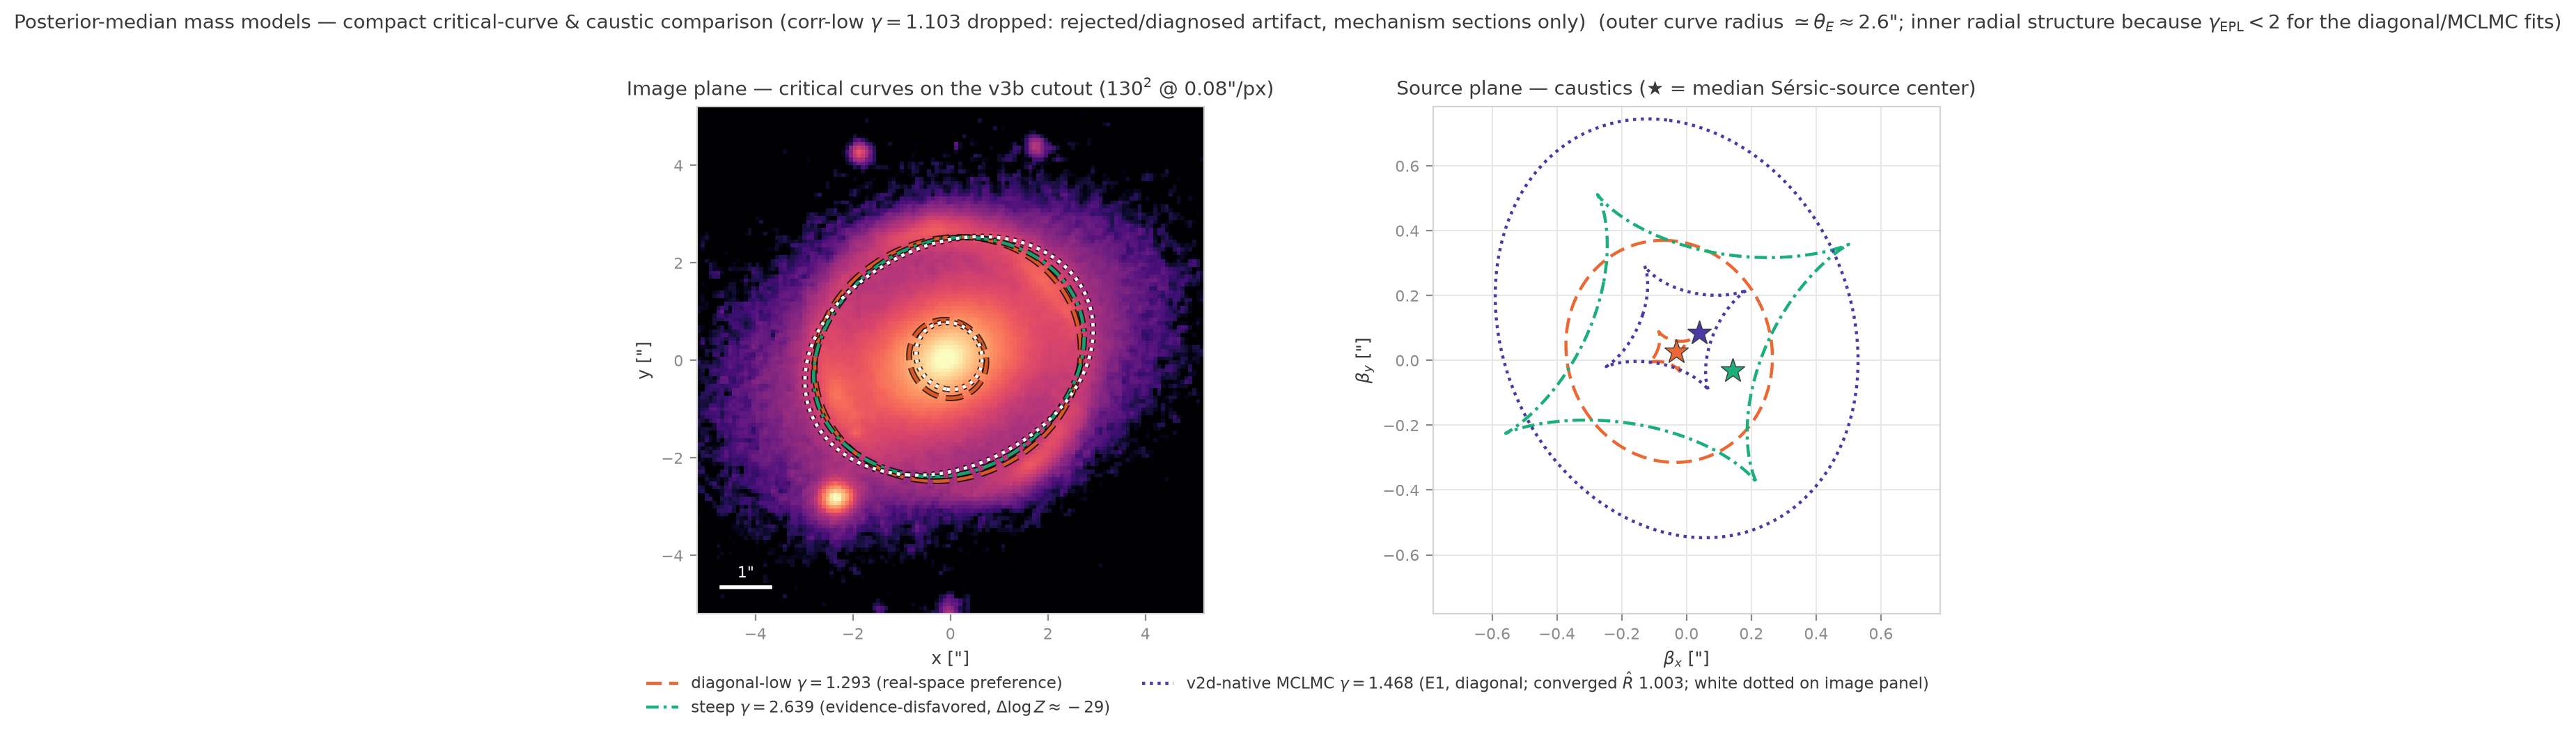
\includegraphics[width=0.98\textwidth]{../figs/rfig_critcurves.png}
\caption{Critical curves (lens plane, over the \dfile{v3b} binned cutout,
asinh stretch) and caustics (source plane; stars mark the median
S\'ersic-source centers) for the three posterior-median mass models,
following the critical-curve/caustic display conventions of the team's
\gigalens\ discovery paper \citep{gu2022gigalens}: corr-low
$\gammaEPL=1.103$ (the certified but artifact-diagnosed correlated fit),
diagonal-low $\gammaEPL=1.293$ (the real-space preference), and steep
$\gammaEPL=2.639$ (evidence-disfavored, $\dlogZ\approx-29$). Scale sanity:
the outer critical curve's median radius matches each model's \thetaE\ to
$<5\%$ (money model: $2.632''$ vs.\ $\thetaE=2.624''$), and the two
shallow ($\gammaEPL<2$) models show the expected inner radial critical
curve and caustic. Deflections from the vendored \sceneapi\ EPL(50)+shear
at the certified conventions; source artifact
\dfile{data/rfig\_modeler\_params.npz}.}
\label{fig:critcurves}
\end{figure}

\paragraph{(2) Reduced $\chi^2$ of the best-fit models.}
Table~\ref{tab:gof-modelers} gives both currencies. Under its own
production metric the money fit is formally excellent: whitened
$\chi^2/\mathrm{dof} = 8946.8/9273 = 0.965$ ($0.973$ after subtracting the
46 nonlinear + 28 marginalized-amplitude
parameters).\footnote{Source artifact:
\dfile{data/summary\_rchi2\_whitened\_corrlow.json} --- recomputed for this
section at the identical posterior-median model point on the validated
stack; it bit-matches the head-to-head artifact's $\gammaEPL$ and whitened
$\log L$ before being quoted.}
Two honest qualifiers frame the real-space column. First, \emph{this
field's own-model floor is $\approx1.6$, not $1.0$}: the injection-build
gate showed that even a ground-truth model of an injected scene scores
$\chi^2/\mathrm{px}=1.598$ full-keep versus $0.952$ on the sky subset ---
essentially all of the excess is bright-object scene-subtraction residue
(bright-object subset $2.71$, lens-center $r<1.2''$ subset
$5.46$)\art{data/t11\_injection\_build\_report.json;
data/t11b\_residue\_mask\_report.json;
data/t04\_realspace\_headtohead.json} --- so the diagonal-low value
$1.578$ \emph{is} the attainable field level, while $7.4$--$8.3$ for the
anchor and money models is genuine real-space misfit (the anchor row also
carries a cross-product resolution handicap: the same parameters render
$\chi^2/\mathrm{px}=1.251$ on their home native product). Second, the
whitened $0.965$ inherits the whitened metric's known caveat: its
stationary kernel class is \emph{rejected} by the field at calibrated
$p=0.010$ (\S\ref{sec:t041}), and the same metric prefers the money model
over diagonal-low by $+63$~nats in $\log L$ ($+501$ in log-posterior),
inverting the real-space ordering --- a reduced $\chi^2$ of $0.965$ here
certifies internal consistency, not noise-model correctness.

\begin{table}[htbp]
\centering
\caption{Goodness of fit for the three best-fit models on the same
\dfile{v3b} binned pixels: real-space $\chi^2/\mathrm{px}$
(diagonal-solved amplitudes; 16{,}653 keep px full field, 7{,}825 px arc
band $r\in[1.2,4.2]''$) and, for the production correlated fit, the
whitened reduced $\chi^2$ over the 9{,}273 whitened dof. Whitened
$\log L$ for all three models is in Table~\ref{tab:headtohead}. Sources:
\dfile{data/t04\_realspace\_headtohead.json},
\dfile{data/summary\_rchi2\_whitened\_corrlow.json},
\dfile{data/t11\_injection\_build\_report.json}.}
\label{tab:gof-modelers}
\small
\begin{tabular}{lccc}
\toprule
model ($\gammaEPL$) & $\chi^2/\mathrm{px}$ full & $\chi^2/\mathrm{px}$ arc
band & whitened $\chi^2/\mathrm{dof}$ \\
\midrule
diag-low $1.293$ (home reference) & $\mathbf{1.578}$ & $\mathbf{1.929}$ & --- \\
anchor $1.433$ (from \dfile{v2d}; home $1.251$) & $7.436$ & $3.622$ & --- \\
corr-low $1.103$ (money) & $8.321$ & $2.756$ & $\mathbf{0.965}$ \\
\midrule
\multicolumn{4}{@{}l@{}}{\footnotesize field's own-model floor (truth model
of injected scene): full-keep $1.598$; sky subset $0.952$ ---} \\
\multicolumn{4}{@{}l@{}}{\footnotesize the excess over $1.0$ is
bright-object scene-subtraction residue, faced by every fit on this
product.} \\
\bottomrule
\end{tabular}
\end{table}

\paragraph{(3) Sampling method.}
In HMC-vs-MCLMC vocabulary: every headline fit in this report was sampled
by \emph{adaptive tempered SMC} \citep{delmoral2006smc} ($\lambda:0\to1$,
per-stage adaptive step targeting a weighted ESS of $0.7N$, per-stage
bootstrap \logZ) whose mutation kernel is \emph{MAMS --- the
Metropolis-adjusted variant of MCLMC}
\citep{robnik2023mclmc,robnik2024mams}: microcanonical (MCLMC) dynamics
made exact by a Metropolis accept/reject step, tuned to the MAMS paper's
target acceptance of $0.90$. It is therefore neither plain HMC nor raw
(unadjusted) MCLMC. The distinction is load-bearing: unadjusted-MCLMC
mutations were demoted at the correctness gate ($20.1\sigma$ evidence bias
on the ill-conditioned analytic target; a measured $\times56$ minor-mode
evidence inflation on the 74-d bimodal target), and everywhere the classic
single-stage MAP$\to$SVI$\to$HMC recipe ran in this campaign it failed its
own acceptance rule (Table~\ref{tab:conv-modelers}; full decision matrix
Table~\ref{tab:decision}, \S\ref{sec:matrix:classic},
\S\ref{sec:matrix:b3}) --- consistent with the companion finding that
these real lens posteriors need the two-stage re-preconditioned recipe
\citep{cgl2026companion}.

\paragraph{(4) Convergence metrics.}
SMC has no $\Rhat$; the honest analogues are independent-seed repeats,
the per-stage weighted-ESS floor maintained by the adaptive
$\lambda$-schedule, unique-particle retention after resampling, MAMS
acceptance against its $0.90$ target, and --- strongest of all --- the
cross-stack, cross-machine reproduction. Table~\ref{tab:conv-modelers} is
the consolidated convergence ledger for every fit quoted in this report,
with $\Rhat$/ESS given where classic MCMC arms ran (both are rejections,
reported as such). For the two inherited diagonal fits (anchor $1.433$,
diag-low $1.293$) the per-fit $\Rhat$/ESS live in the companion report's
campaign ledger \citep{cgl2026companion} and are cited, not re-derived
here. Table~\ref{tab:conv-modelers} covers the fits \emph{quoted} in this
report; Appendix~\ref{app:convergence} extends it to the complete per-fit
ledger --- one row for every fit the campaign ever ran, including the
failed, rejected, collapsed, and budget-blocked arms.

\begin{table}[htbp]
\centering
\caption{Consolidated convergence ledger. wESS = final-stage weighted ESS;
``unique'' = unique particles after resampling; the adaptive
$\lambda$-schedule holds per-stage wESS at $0.7N$ by construction. Sources:
\dfile{data/t02\_t03\_gate\_eval.json} (+ per-seed run JSONs),
\dfile{data/results-perlmutter/l0g2\_v3b\_scene\_seed2.json},
\dfile{data/b1r\_decision\_matrix.json} +
\dfile{research/checkpoint\_b1r\_close.md},
\dfile{data/results-perlmutter/l0\_arbitration\_classic.json},
\dfile{data/b3\_run\_ref\_sys\{0..3\}\_l4-8.json},
\citet{cgl2026companion}.}
\label{tab:conv-modelers}
\scriptsize
\setlength{\tabcolsep}{3.5pt}
\renewcommand{\arraystretch}{1.3}
\begin{tabular}{@{}p{0.21\textwidth}p{0.135\textwidth}p{0.37\textwidth}p{0.21\textwidth}@{}}
\toprule
fit / arm & vehicle, $n$ & diagnostics & verdict \\
\midrule
\dfile{v3b} corr \textbf{low} ---
$\gammaEPL=1.1032\pm0.0086$ (\textbf{money}) &
tempered SMC + MAMS; 3 seeds $\times$ 128 &
$\lambda{=}1$ @28 stages every seed; wESS 118--128/128; unique 77--82/128;
seeds $\{1.1032, 1.0967, 1.1005\}$ $\Rightarrow$
$\sseed(\gammaEPL)=0.00325$, $\sseed(\logZ)=1.22$ nats &
\textbf{converged + seed-certified} (T0.2, \S\ref{sec:t02}); $n{=}3$
caveat: $\pm46\%$ on $\sseed$ itself \\
\dfile{v3b} corr steep ($\gammaEPL\approx2.64$) &
same; 3 seeds $\times$ 96 &
$\lambda{=}1$ @21--22 stages; wESS 36--96/96 (seed-2 final resample low);
unique 50--59/96; $\sseed(\gammaEPL)=0.00664$ &
converged; $\dlogZ(\mathrm{steep}-\mathrm{low})=-28.9/-32.3/-31.2$
seed-stable \\
same fit, \sceneapi\ port, Perlmutter A100 (L0-G2) &
same; 1 seed &
$\lambda{=}1$ @27/22 stages; wESS 123.5/128 (low), 47.6/96 (steep);
unique 81/128, 54/96 &
\textbf{PASS}: $\Delta\gammaEPL=0.0027$; \logZ\ agreement 0.11
(low)\,/\,0.37 (steep) nats \emph{across stacks and machines}
(\S\ref{sec:l0g2}) \\
carousel 33-d multi-plane REAL (B1r; hardest cell) &
same; 1 seed $\times$ 128 &
$\lambda=0.151$ @36 stages; unique 92--104/128 every stage; MAMS accept
0.871--0.934 (mean 0.899 vs 0.90 target); stage wESS pinned at $0.7N$ &
\textbf{no posterior}: sampler healthy, killed by wall-cap --- a cost
verdict, not a convergence failure (\S\ref{sec:matrix:b1r}) \\
\midrule
classic MAP$\to$SVI$\to$HMC, warm, \dfile{v2d} (arbitration arm) &
50 chains, 250 burn-in/750 draws; escalated 500/1500 &
$\Rhat_{\rm worst}=44.3$ (escalated $11.7$) vs rule $<1.05$;
$\ESS_{\min}=53.6$ ($63.0$ escalated); all chains railed
$\gammaEPL\approx1.987\,[1.983,1.991]$ at the prior edge &
\textbf{NO-VERDICT}: $\gammaEPL$ not quotable; reproduces the known T2
single-stage pathology on the \sceneapi\ (\S\ref{sec:matrix:classic}) \\
classic reference chains, hs2 scenes $\times4$ (B3) &
frozen 50-chain recipe &
$\Rhat_{\rm worst}=4.36$--$7.87$; $\ESS_{\min}=63.7$--$83.9$ vs rule
$\Rhat<1.05 \wedge \ESS\ge200$ &
all 4 \textbf{rejected} by the pre-registered acceptance rule
(\S\ref{sec:matrix:b3}) \\
\midrule
anchor $1.433$ (\dfile{v2d} diag) and diag-low $1.293$ (\dfile{v3b} diag) &
companion campaign (two-stage re-preconditioned recipe) &
provenance row: per-fit $\Rhat$/\ESS\ ledgered in the companion report &
converged there; cited, not re-derived \citep{cgl2026companion} \\
\bottomrule
\end{tabular}
\end{table}

\paragraph{(5) The posterior.}
Figure~\ref{fig:corner} shows the posterior corner for the production
correlated \dfile{v3b} fit with the three seed repeats overlaid. The
read-out: the Einstein radius is tight and stable
($\thetaE=2.6239\pm0.0049$, a $0.2\%$ constraint) while the two basins
remain cleanly separated in $\gammaEPL$ (low $1.103$ vs.\ steep $2.64$)
with a seed-stable evidence preference for the low basin of
$\approx29$--$32$ nats; the seed overlays coincide within
$\sseed(\gammaEPL)=0.00325$, which is what licenses quoting
$\sigma_{\rm tot}=0.0086$ on the money number
(\S\ref{sec:t02}).\footnote{Source artifacts: companion
\dfile{data/results/e2\_v3b\_low\_smc\_canary\_fix.json};
\dfile{data/t02\_t03\_gate\_eval.json}.}
The number this posterior constrains, and the standing caveat on
interpreting it, are the subject of the rest of this report:
$\gammaEPL=1.1032\pm0.0086$ is certified, cross-stack reproduced --- and
diagnosed as an artifact of a stationary noise-model class the field
rejects.

\begin{figure}[htbp]
\centering
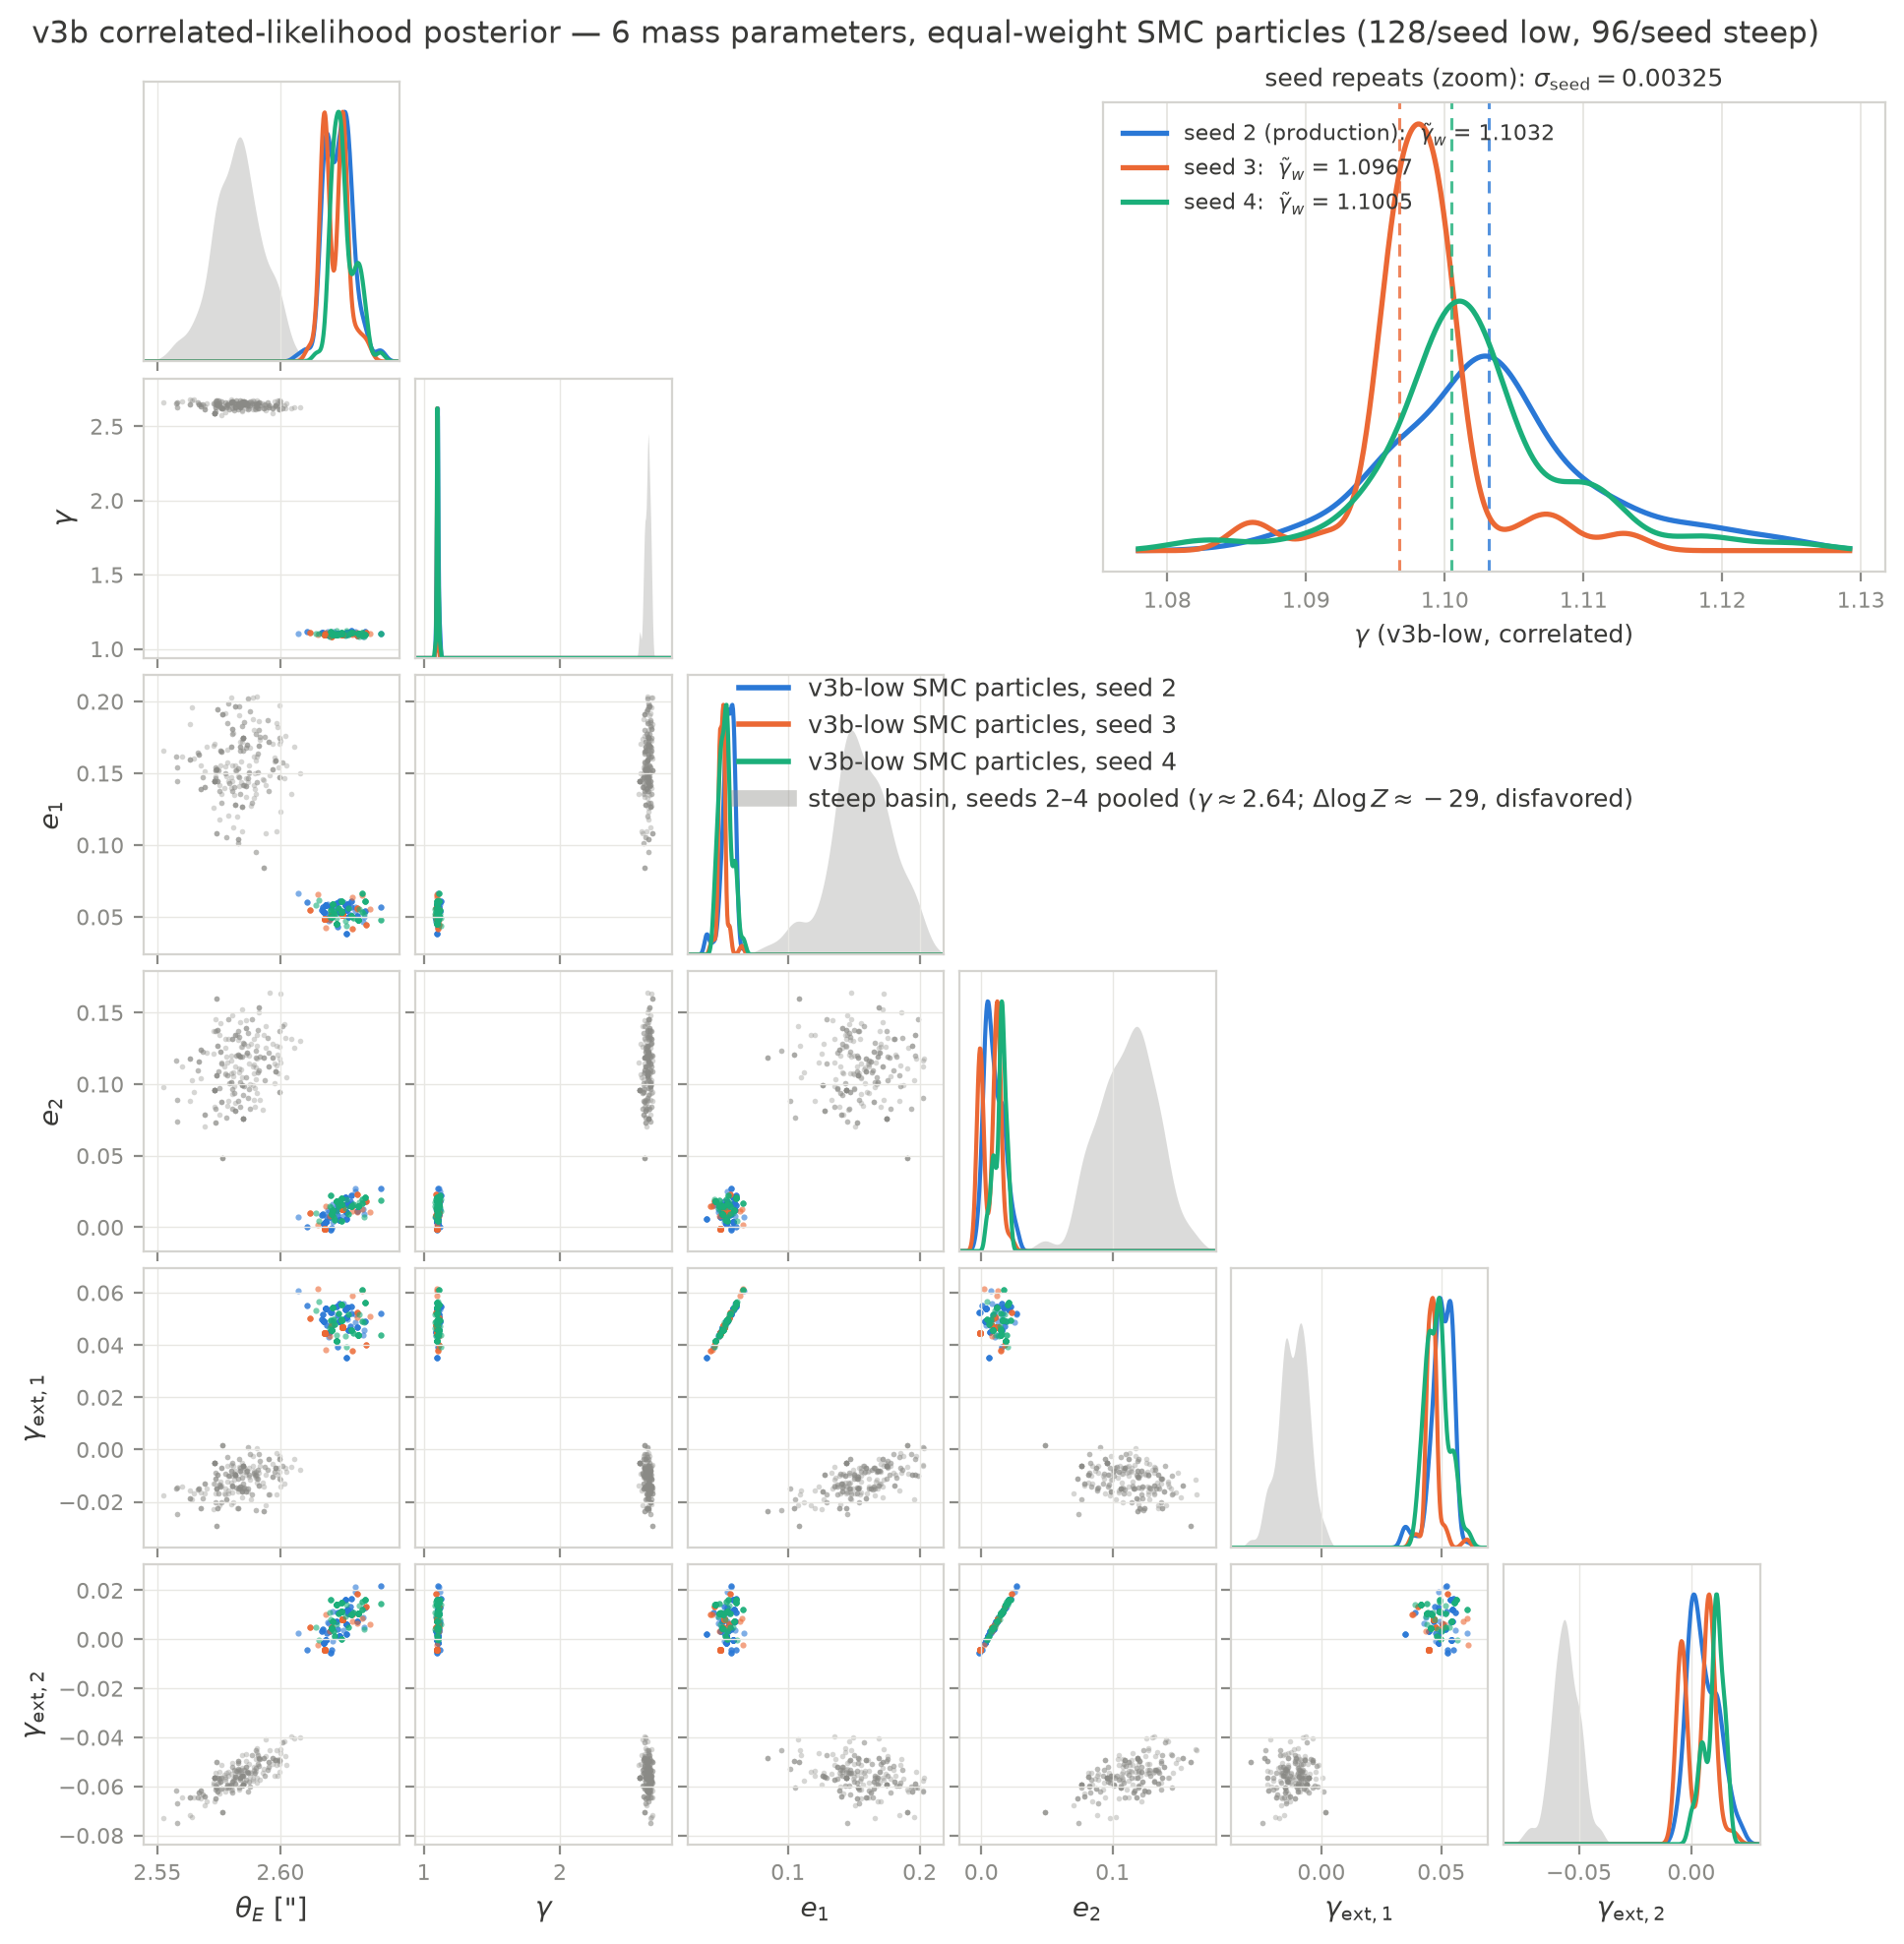
\includegraphics[width=0.98\textwidth]{../figs/rfig_corner.png}
\caption{Posterior corner of the six mass parameters (\thetaE,
$\gammaEPL$, \eone, \etwo, $\gamma_{\mathrm{ext},1}$,
$\gamma_{\mathrm{ext},2}$) from the stored equal-weight \dfile{v3b}-low
correlated SMC particles, seeds $\{2,3,4\}$ overlaid --- the SMC
convergence visual (SMC has no \Rhat; the seed-repeat spread
$\sseed=0.00325$ plus the per-stage ESS/acceptance diagnostics of
Table~\ref{tab:conv-modelers} are the analogues). Grey: the steep basin
(seeds 2--4 pooled, $\gammaEPL\approx2.64$; evidence-disfavored by
$\approx29$--$32$ nats). Inset: $\gammaEPL$ zoom with the per-seed
weighted medians of record $\{1.1032, 1.0967, 1.1005\}$; the equal-weight
particle medians reproduce them to $\le0.0027$, well inside
$\sigma_{\rm stat}=0.008$. Source artifacts: companion
\dfile{data/results/e2\_v3b\_low\_smc\_canary\_fix.json} (+ seed-3/4
repeats), \dfile{data/t02\_t03\_gate\_eval.json},
\dfile{data/rfig\_modeler\_params.npz}.}
\label{fig:corner}
\end{figure}
